\PassOptionsToPackage{unicode=true}{hyperref} % options for packages loaded elsewhere
\PassOptionsToPackage{hyphens}{url}
%
\documentclass[]{article}
\usepackage{lmodern}
\usepackage{amssymb,amsmath}
\usepackage{ifxetex,ifluatex}
\usepackage{fixltx2e} % provides \textsubscript
\ifnum 0\ifxetex 1\fi\ifluatex 1\fi=0 % if pdftex
  \usepackage[T1]{fontenc}
  \usepackage[utf8]{inputenc}
  \usepackage{textcomp} % provides euro and other symbols
\else % if luatex or xelatex
  \usepackage{unicode-math}
  \defaultfontfeatures{Ligatures=TeX,Scale=MatchLowercase}
\fi
% use upquote if available, for straight quotes in verbatim environments
\IfFileExists{upquote.sty}{\usepackage{upquote}}{}
% use microtype if available
\IfFileExists{microtype.sty}{%
\usepackage[]{microtype}
\UseMicrotypeSet[protrusion]{basicmath} % disable protrusion for tt fonts
}{}
\IfFileExists{parskip.sty}{%
\usepackage{parskip}
}{% else
\setlength{\parindent}{0pt}
\setlength{\parskip}{6pt plus 2pt minus 1pt}
}
\usepackage{hyperref}
\hypersetup{
            pdftitle={Lenguaje de programación y testeo estadístico: El caso de Ventanas},
            pdfauthor={Vera Sativa},
            pdfborder={0 0 0},
            breaklinks=true}
\urlstyle{same}  % don't use monospace font for urls
\usepackage[lmargin=20mm,rmargin=20mm,tmargin=18mm,bmargin=22mm]{geometry}
\usepackage{longtable,booktabs}
% Fix footnotes in tables (requires footnote package)
\IfFileExists{footnote.sty}{\usepackage{footnote}\makesavenoteenv{longtable}}{}
\usepackage{graphicx,grffile}
\usepackage[labelformat=empty]{caption}
\usepackage{etoolbox}
\makeatletter
\def\maxwidth{\ifdim\Gin@nat@width>\linewidth\linewidth\else\Gin@nat@width\fi}
\def\maxheight{\ifdim\Gin@nat@height>\textheight\textheight\else\Gin@nat@height\fi}
\patchcmd{\@verbatim}
  {\verbatim@font}
  {\verbatim@font\small}
  {}{}
\makeatother
% Scale images if necessary, so that they will not overflow the page
% margins by default, and it is still possible to overwrite the defaults
% using explicit options in \includegraphics[width, height, ...]{}
\setkeys{Gin}{width=\maxwidth,height=\maxheight,keepaspectratio}
% Make links footnotes instead of hotlinks:
\DeclareRobustCommand{\href}[2]{#2\footnote{\url{#1}}}
\setlength{\emergencystretch}{3em}  % prevent overfull lines
\providecommand{\tightlist}{%
  \setlength{\itemsep}{0pt}\setlength{\parskip}{0pt}}
\setcounter{secnumdepth}{0}
% Redefines (sub)paragraphs to behave more like sections
\ifx\paragraph\undefined\else
\let\oldparagraph\paragraph
\renewcommand{\paragraph}[1]{\oldparagraph{#1}\mbox{}}
\fi
\ifx\subparagraph\undefined\else
\let\oldsubparagraph\subparagraph
\renewcommand{\subparagraph}[1]{\oldsubparagraph{#1}\mbox{}}
\fi

% set default figure placement to htbp
\makeatletter
\def\fps@figure{htbp}
\makeatother


\title{Lenguaje de programación y testeo estadístico: El caso de Ventanas}
\providecommand{\subtitle}[1]{}
\subtitle{Una comparativa entre la zona crítica y resto de Chile}
\author{Vera Sativa\footnote{Corresponding author – hola@verasativa.com}}
\date{\today}

\begin{document}
\maketitle
\begin{abstract}
Utilizando el lenguaje de programación Python, tras unificar los
registros anuales de defunciones en Chile 1998-2016
(\textasciitilde{}1.7M), analizamos los diagnósticos primarios en
defunciones de menores hasta 16 años, comparando la zona crítica bajo la
contaminación del complejo industrial Quintero-Ventanas, contra el resto
de Chile como control. Encontramos incidencias de malformaciones
congénitas, deformidades y anomalías cromosómicas (CIE-10: Q00-Q99),
3.04 a 3.75 desviaciones estándar sobre el resto del país, con P-values
de 0.0001 a 0.00002 en un millón de simulaciones, estimando un impacto
de entre 29.73 a 37.8 muertes de menores en la zona crítica por sobre la
norma nacional. La metodología podría ser escalada a todo el país para
detectar focos de contaminación desconocidos.
\end{abstract}

\hypertarget{una-comparativa-entre-la-zona-cruxedtica-y-el-resto-de-chile}{%
\subsection{Una comparativa entre la zona crítica y el resto de
Chile}\label{una-comparativa-entre-la-zona-cruxedtica-y-el-resto-de-chile}}

\hypertarget{introducciuxf3n}{%
\subsubsection{Introducción}\label{introducciuxf3n}}

Mediante programación en \emph{Python} fue posible estandarizar los
registros de defunciones oficiales, que tienen una serie de variaciones
año a año. Una vez construido un \emph{registro
unificado de defunciones en Chile, entre el año 1998 y 2016}\textsuperscript{{1}}, surge la
pregunta general: ¿Se podrán observar en éste, rasgos distintos en una
zona crítica al resto de Chile? Utilizando el mismo lenguaje de
programación testearemos esa hipótesis.

Un aporte clave es la metodología, y por esta razón se disponibiliza todo el \emph{código fuente}\textsuperscript{{2}}, posibilitando la implementación y extensión de ésta en otros problemas, territorios o datasets. 

\hypertarget{antecedentes}{%
\subsubsection{Antecedentes}\label{antecedentes}}

El impacto ambiental y sobre la salud humana del complejo industrial
Quintero-Ventanas ha sido ampliamente documentado al punto de que recientemente el Colegio Medico chileno dedicó un número completo de su revista de salud
pública \emph{Cuadernos Médico Sociales} al problema\textsuperscript{{3}}

El reciente informe \emph{The Lancet Commission on Pollution and Health}
señala que la polución del aire puede ser vinculada al aumento de
nacimientos prematuros y con bajo peso. Y que algunos estudios han
mostrado asociación entre polución ambiental del aire y aumento del
riesgo de síndrome de muerte súbita del lactante\textsuperscript{{4}}.

\hypertarget{comparaciuxf3n-de-diagnuxf3sticos-primarios}{%
\subsubsection{Comparación de diagnósticos
primarios}\label{comparaciuxf3n-de-diagnuxf3sticos-primarios}}

Para buscar una respuesta a la asociación entre contaminación ambiental y enfermedades de la gestación, es posible usar con todas sus limitaciones los registros de defunciones oficiales del país. Una forma de avanzar por sobre esas restricciones es hacer uso de \emph{la integración jerárquica de los códigos de diagnóstico CIE-10}\textsuperscript{{5}}  en el dataset. Una comparación de éstos se presenta como la
opción más evidente y atractiva, mediante un trabajo de programación en Phyton. Este trabajo desarrolla una metodología de programación orientada al objeto de estudio y pone a Phyton como una alternativa para su uso en salud pública.

\hypertarget{limitaciones de los datos}{%
\subsubsection{Limitaciones de los datos}\label{limitaciones}}

Para entender que podemos investigar desde estos datos, debemos reconocer sus limitaciones. Dado que este dataset solo incluye las defunciones y no contiene
información sobre la población general, no es posible hacer un análisis
respecto a tasas de ocurrencia sin tener que usar datos
como censos. La ruralidad de la zona, conjugada con la migración
campo-ciudad, produce un movimiento poblacional que en ese período aumenta la incertidumbre de las cifras. Tampoco podemos hacer un
análisis sobre la distribución etaria de la mortalidad, ni la
distribución de diagnósticos primarios en la población general, sin
normalizar primero con datos adicionales.

\hypertarget{pregunta-de-investigaciuxf3n}{%
\subsubsection{Pregunta de
investigación}\label{pregunta-de-investigaciuxf3n}}

Con esas limitaciones en mente, podemos plantear una pregunta sencilla,
pero contestable:

\textbf{¿Cómo se comparan los diagnósticos primarios de defunciones, en
la zona de interés, con respecto al resto del país en menores de 16
años?}

\hypertarget{proceso-exploratorio-definiendo-la-zona-de-interuxe9s}{%
\subsubsection{Proceso exploratorio: definiendo la ``zona de
interés''}\label{proceso-exploratorio-definiendo-la-zona-de-interuxe9s}}

Inicialmente, se exploró como zona de interés solamente las comunas de
Quintero y Puchuncaví, puesto que son colindantes (Quintero) o el lugar mismo del
foco industrial de contaminación .

\begin{verbatim}
Zona de interés: Quintero, Puchuncaví
Total defunciones en el grupo de interés: 119
Total defunciones en los 10 principales diagnósticos primarios del grupo de interés: 118
Fracción del total: 0.992
\end{verbatim}

\begin{figure}
\centering
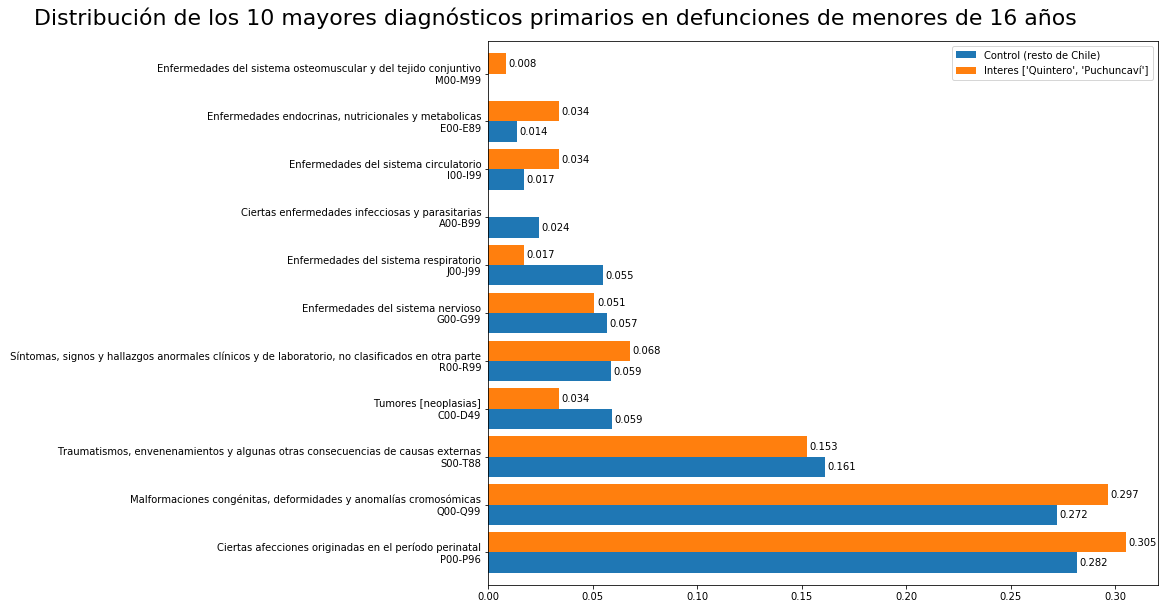
\includegraphics{assets/10-diagnosticos-(Quintero-Puchuncavi).png}
\caption{Figura 1: Distribución de los 10 mayores diagnósticos primarios en defunciones de menores hasta 16 años (Quintero-Puchuncaví)}
\end{figure}

Sin embargo, no se econtró algo claro ya que podemos observar en la figura 1 que hay dos diagnósticos
primarios que presentan incidencias superiores a la nacional. Con la
intención de buscar una tendencia más clara y validable (tamaño de la
muestra), exploramos la incidencia de estos dos diagnósticos primarios
en todas las comunas de la Quinta Región.

\hypertarget{ciertas-afecciones-originadas-en-el-peruxedodo-perinatal-p00-p96}{%
\subsubsection{Ciertas afecciones originadas en el período perinatal
(P00-P96)}\label{ciertas-afecciones-originadas-en-el-peruxedodo-perinatal-p00-p96}}

\begin{longtable}[]{@{}llllllll@{}}
\toprule
\begin{minipage}[b]{0.03\columnwidth}\raggedright
\#\strut
\end{minipage} & \begin{minipage}[b]{0.09\columnwidth}\raggedright
Comuna\strut
\end{minipage} & \begin{minipage}[b]{0.14\columnwidth}\raggedright
Incidencia comuna\strut
\end{minipage} & \begin{minipage}[b]{0.13\columnwidth}\raggedright
Incidencia otros\strut
\end{minipage} & \begin{minipage}[b]{0.10\columnwidth}\raggedright
Proporción comuna\strut
\end{minipage} & \begin{minipage}[b]{0.09\columnwidth}\raggedright
Proporción otros\strut
\end{minipage} & \begin{minipage}[b]{0.11\columnwidth}\raggedright
Total comuna\strut
\end{minipage} & \begin{minipage}[b]{0.10\columnwidth}\raggedright
Total otros\strut
\end{minipage}\tabularnewline
\midrule
\endhead
\begin{minipage}[t]{0.03\columnwidth}\raggedright
0\strut
\end{minipage} & \begin{minipage}[t]{0.09\columnwidth}\raggedright
La Cruz\strut
\end{minipage} & \begin{minipage}[t]{0.14\columnwidth}\raggedright
26\strut
\end{minipage} & \begin{minipage}[t]{0.13\columnwidth}\raggedright
15957\strut
\end{minipage} & \begin{minipage}[t]{0.10\columnwidth}\raggedright
0.509804\strut
\end{minipage} & \begin{minipage}[t]{0.09\columnwidth}\raggedright
0.274836\strut
\end{minipage} & \begin{minipage}[t]{0.11\columnwidth}\raggedright
51\strut
\end{minipage} & \begin{minipage}[t]{0.10\columnwidth}\raggedright
58060\strut
\end{minipage}\tabularnewline
\begin{minipage}[t]{0.03\columnwidth}\raggedright
1\strut
\end{minipage} & \begin{minipage}[t]{0.09\columnwidth}\raggedright
Rinconada\strut
\end{minipage} & \begin{minipage}[t]{0.14\columnwidth}\raggedright
15\strut
\end{minipage} & \begin{minipage}[t]{0.13\columnwidth}\raggedright
15968\strut
\end{minipage} & \begin{minipage}[t]{0.10\columnwidth}\raggedright
0.46875\strut
\end{minipage} & \begin{minipage}[t]{0.09\columnwidth}\raggedright
0.274936\strut
\end{minipage} & \begin{minipage}[t]{0.11\columnwidth}\raggedright
32\strut
\end{minipage} & \begin{minipage}[t]{0.10\columnwidth}\raggedright
58079\strut
\end{minipage}\tabularnewline
\begin{minipage}[t]{0.03\columnwidth}\raggedright
2\strut
\end{minipage} & \begin{minipage}[t]{0.09\columnwidth}\raggedright
San Felipe\strut
\end{minipage} & \begin{minipage}[t]{0.14\columnwidth}\raggedright
109\strut
\end{minipage} & \begin{minipage}[t]{0.13\columnwidth}\raggedright
15874\strut
\end{minipage} & \begin{minipage}[t]{0.10\columnwidth}\raggedright
0.37457\strut
\end{minipage} & \begin{minipage}[t]{0.09\columnwidth}\raggedright
0.274542\strut
\end{minipage} & \begin{minipage}[t]{0.11\columnwidth}\raggedright
291\strut
\end{minipage} & \begin{minipage}[t]{0.10\columnwidth}\raggedright
57820\strut
\end{minipage}\tabularnewline
\begin{minipage}[t]{0.03\columnwidth}\raggedright
3\strut
\end{minipage} & \begin{minipage}[t]{0.09\columnwidth}\raggedright
Olmué\strut
\end{minipage} & \begin{minipage}[t]{0.14\columnwidth}\raggedright
17\strut
\end{minipage} & \begin{minipage}[t]{0.13\columnwidth}\raggedright
15966\strut
\end{minipage} & \begin{minipage}[t]{0.10\columnwidth}\raggedright
0.369565\strut
\end{minipage} & \begin{minipage}[t]{0.09\columnwidth}\raggedright
0.274968\strut
\end{minipage} & \begin{minipage}[t]{0.11\columnwidth}\raggedright
46\strut
\end{minipage} & \begin{minipage}[t]{0.10\columnwidth}\raggedright
58065\strut
\end{minipage}\tabularnewline
\begin{minipage}[t]{0.03\columnwidth}\raggedright
4\strut
\end{minipage} & \begin{minipage}[t]{0.09\columnwidth}\raggedright
El Tabo\strut
\end{minipage} & \begin{minipage}[t]{0.14\columnwidth}\raggedright
7\strut
\end{minipage} & \begin{minipage}[t]{0.13\columnwidth}\raggedright
15976\strut
\end{minipage} & \begin{minipage}[t]{0.10\columnwidth}\raggedright
0.368421\strut
\end{minipage} & \begin{minipage}[t]{0.09\columnwidth}\raggedright
0.275012\strut
\end{minipage} & \begin{minipage}[t]{0.11\columnwidth}\raggedright
19\strut
\end{minipage} & \begin{minipage}[t]{0.10\columnwidth}\raggedright
58092\strut
\end{minipage}\tabularnewline
\begin{minipage}[t]{0.03\columnwidth}\raggedright
5\strut
\end{minipage} & \begin{minipage}[t]{0.09\columnwidth}\raggedright
San Esteban\strut
\end{minipage} & \begin{minipage}[t]{0.14\columnwidth}\raggedright
15\strut
\end{minipage} & \begin{minipage}[t]{0.13\columnwidth}\raggedright
15968\strut
\end{minipage} & \begin{minipage}[t]{0.10\columnwidth}\raggedright
0.357143\strut
\end{minipage} & \begin{minipage}[t]{0.09\columnwidth}\raggedright
0.274983\strut
\end{minipage} & \begin{minipage}[t]{0.11\columnwidth}\raggedright
42\strut
\end{minipage} & \begin{minipage}[t]{0.10\columnwidth}\raggedright
58069\strut
\end{minipage}\tabularnewline
\begin{minipage}[t]{0.03\columnwidth}\raggedright
6\strut
\end{minipage} & \begin{minipage}[t]{0.09\columnwidth}\raggedright
Cartagena\strut
\end{minipage} & \begin{minipage}[t]{0.14\columnwidth}\raggedright
18\strut
\end{minipage} & \begin{minipage}[t]{0.13\columnwidth}\raggedright
15965\strut
\end{minipage} & \begin{minipage}[t]{0.10\columnwidth}\raggedright
0.339623\strut
\end{minipage} & \begin{minipage}[t]{0.09\columnwidth}\raggedright
0.274984\strut
\end{minipage} & \begin{minipage}[t]{0.11\columnwidth}\raggedright
53\strut
\end{minipage} & \begin{minipage}[t]{0.10\columnwidth}\raggedright
58058\strut
\end{minipage}\tabularnewline
\begin{minipage}[t]{0.03\columnwidth}\raggedright
7\strut
\end{minipage} & \begin{minipage}[t]{0.09\columnwidth}\raggedright
Llaillay\strut
\end{minipage} & \begin{minipage}[t]{0.14\columnwidth}\raggedright
28\strut
\end{minipage} & \begin{minipage}[t]{0.13\columnwidth}\raggedright
15955\strut
\end{minipage} & \begin{minipage}[t]{0.10\columnwidth}\raggedright
0.337349\strut
\end{minipage} & \begin{minipage}[t]{0.09\columnwidth}\raggedright
0.274953\strut
\end{minipage} & \begin{minipage}[t]{0.11\columnwidth}\raggedright
83\strut
\end{minipage} & \begin{minipage}[t]{0.10\columnwidth}\raggedright
58028\strut
\end{minipage}\tabularnewline
\begin{minipage}[t]{0.03\columnwidth}\raggedright
8\strut
\end{minipage} & \begin{minipage}[t]{0.09\columnwidth}\raggedright
Calle Larga\strut
\end{minipage} & \begin{minipage}[t]{0.14\columnwidth}\raggedright
13\strut
\end{minipage} & \begin{minipage}[t]{0.13\columnwidth}\raggedright
15970\strut
\end{minipage} & \begin{minipage}[t]{0.10\columnwidth}\raggedright
0.333333\strut
\end{minipage} & \begin{minipage}[t]{0.09\columnwidth}\raggedright
0.275003\strut
\end{minipage} & \begin{minipage}[t]{0.11\columnwidth}\raggedright
39\strut
\end{minipage} & \begin{minipage}[t]{0.10\columnwidth}\raggedright
58072\strut
\end{minipage}\tabularnewline
\begin{minipage}[t]{0.03\columnwidth}\raggedright
9\strut
\end{minipage} & \begin{minipage}[t]{0.09\columnwidth}\raggedright
Algarrobo\strut
\end{minipage} & \begin{minipage}[t]{0.14\columnwidth}\raggedright
11\strut
\end{minipage} & \begin{minipage}[t]{0.13\columnwidth}\raggedright
15972\strut
\end{minipage} & \begin{minipage}[t]{0.10\columnwidth}\raggedright
0.323529\strut
\end{minipage} & \begin{minipage}[t]{0.09\columnwidth}\raggedright
0.275014\strut
\end{minipage} & \begin{minipage}[t]{0.11\columnwidth}\raggedright
34\strut
\end{minipage} & \begin{minipage}[t]{0.10\columnwidth}\raggedright
58077\strut
\end{minipage}\tabularnewline
\begin{minipage}[t]{0.03\columnwidth}\raggedright
10\strut
\end{minipage} & \begin{minipage}[t]{0.09\columnwidth}\raggedright
Quintero\strut
\end{minipage} & \begin{minipage}[t]{0.14\columnwidth}\raggedright
23\strut
\end{minipage} & \begin{minipage}[t]{0.13\columnwidth}\raggedright
15960\strut
\end{minipage} & \begin{minipage}[t]{0.10\columnwidth}\raggedright
0.315068\strut
\end{minipage} & \begin{minipage}[t]{0.09\columnwidth}\raggedright
0.274992\strut
\end{minipage} & \begin{minipage}[t]{0.11\columnwidth}\raggedright
73\strut
\end{minipage} & \begin{minipage}[t]{0.10\columnwidth}\raggedright
58038\strut
\end{minipage}\tabularnewline
\begin{minipage}[t]{0.03\columnwidth}\raggedright
11\strut
\end{minipage} & \begin{minipage}[t]{0.09\columnwidth}\raggedright
Hijuelas\strut
\end{minipage} & \begin{minipage}[t]{0.14\columnwidth}\raggedright
23\strut
\end{minipage} & \begin{minipage}[t]{0.13\columnwidth}\raggedright
15960\strut
\end{minipage} & \begin{minipage}[t]{0.10\columnwidth}\raggedright
0.310811\strut
\end{minipage} & \begin{minipage}[t]{0.09\columnwidth}\raggedright
0.274997\strut
\end{minipage} & \begin{minipage}[t]{0.11\columnwidth}\raggedright
74\strut
\end{minipage} & \begin{minipage}[t]{0.10\columnwidth}\raggedright
58037\strut
\end{minipage}\tabularnewline
\bottomrule
\caption{Tabla 1: Incidencias comunales y nacionales de P00-P96}
\end{longtable}

\hypertarget{malformaciones-conguxe9nitas-deformidades-y-anomaluxedas-cromosuxf3micas-q00-q99}{%
\subsubsection{Malformaciones congénitas, deformidades y anomalías
cromosómicas
(Q00-Q99)}\label{malformaciones-conguxe9nitas-deformidades-y-anomaluxedas-cromosuxf3micas-q00-q99}}

\begin{longtable}[]{@{}llllllll@{}}
\toprule
\begin{minipage}[b]{0.03\columnwidth}\raggedright
\#\strut
\end{minipage} & \begin{minipage}[b]{0.09\columnwidth}\raggedright
Comuna\strut
\end{minipage} & \begin{minipage}[b]{0.14\columnwidth}\raggedright
Incidencia comuna\strut
\end{minipage} & \begin{minipage}[b]{0.13\columnwidth}\raggedright
Incidencia otros\strut
\end{minipage} & \begin{minipage}[b]{0.10\columnwidth}\raggedright
Proporción comuna\strut
\end{minipage} & \begin{minipage}[b]{0.09\columnwidth}\raggedright
Proporción otros\strut
\end{minipage} & \begin{minipage}[b]{0.10\columnwidth}\raggedright
Total comuna\strut
\end{minipage} & \begin{minipage}[b]{0.10\columnwidth}\raggedright
Total otros\strut
\end{minipage}\tabularnewline
\midrule
\endhead
\begin{minipage}[t]{0.03\columnwidth}\raggedright
0\strut
\end{minipage} & \begin{minipage}[t]{0.09\columnwidth}\raggedright
Puchuncaví\strut
\end{minipage} & \begin{minipage}[t]{0.14\columnwidth}\raggedright
20\strut
\end{minipage} & \begin{minipage}[t]{0.13\columnwidth}\raggedright
15428\strut
\end{minipage} & \begin{minipage}[t]{0.10\columnwidth}\raggedright
0.434783\strut
\end{minipage} & \begin{minipage}[t]{0.09\columnwidth}\raggedright
0.265702\strut
\end{minipage} & \begin{minipage}[t]{0.10\columnwidth}\raggedright
46\strut
\end{minipage} & \begin{minipage}[t]{0.10\columnwidth}\raggedright
58065\strut
\end{minipage}\tabularnewline
\begin{minipage}[t]{0.03\columnwidth}\raggedright
1\strut
\end{minipage} & \begin{minipage}[t]{0.09\columnwidth}\raggedright
Zapallar\strut
\end{minipage} & \begin{minipage}[t]{0.14\columnwidth}\raggedright
6\strut
\end{minipage} & \begin{minipage}[t]{0.13\columnwidth}\raggedright
15442\strut
\end{minipage} & \begin{minipage}[t]{0.10\columnwidth}\raggedright
0.428571\strut
\end{minipage} & \begin{minipage}[t]{0.09\columnwidth}\raggedright
0.265797\strut
\end{minipage} & \begin{minipage}[t]{0.10\columnwidth}\raggedright
14\strut
\end{minipage} & \begin{minipage}[t]{0.10\columnwidth}\raggedright
58097\strut
\end{minipage}\tabularnewline
\begin{minipage}[t]{0.03\columnwidth}\raggedright
2\strut
\end{minipage} & \begin{minipage}[t]{0.09\columnwidth}\raggedright
Papudo\strut
\end{minipage} & \begin{minipage}[t]{0.14\columnwidth}\raggedright
3\strut
\end{minipage} & \begin{minipage}[t]{0.13\columnwidth}\raggedright
15445\strut
\end{minipage} & \begin{minipage}[t]{0.10\columnwidth}\raggedright
0.375\strut
\end{minipage} & \begin{minipage}[t]{0.09\columnwidth}\raggedright
0.265821\strut
\end{minipage} & \begin{minipage}[t]{0.10\columnwidth}\raggedright
8\strut
\end{minipage} & \begin{minipage}[t]{0.10\columnwidth}\raggedright
58103\strut
\end{minipage}\tabularnewline
\begin{minipage}[t]{0.03\columnwidth}\raggedright
3\strut
\end{minipage} & \begin{minipage}[t]{0.09\columnwidth}\raggedright
La Ligua\strut
\end{minipage} & \begin{minipage}[t]{0.14\columnwidth}\raggedright
37\strut
\end{minipage} & \begin{minipage}[t]{0.13\columnwidth}\raggedright
15411\strut
\end{minipage} & \begin{minipage}[t]{0.10\columnwidth}\raggedright
0.37\strut
\end{minipage} & \begin{minipage}[t]{0.09\columnwidth}\raggedright
0.265657\strut
\end{minipage} & \begin{minipage}[t]{0.10\columnwidth}\raggedright
100\strut
\end{minipage} & \begin{minipage}[t]{0.10\columnwidth}\raggedright
58011\strut
\end{minipage}\tabularnewline
\begin{minipage}[t]{0.03\columnwidth}\raggedright
4\strut
\end{minipage} & \begin{minipage}[t]{0.09\columnwidth}\raggedright
Concón\strut
\end{minipage} & \begin{minipage}[t]{0.14\columnwidth}\raggedright
30\strut
\end{minipage} & \begin{minipage}[t]{0.13\columnwidth}\raggedright
15418\strut
\end{minipage} & \begin{minipage}[t]{0.10\columnwidth}\raggedright
0.352941\strut
\end{minipage} & \begin{minipage}[t]{0.09\columnwidth}\raggedright
0.265708\strut
\end{minipage} & \begin{minipage}[t]{0.10\columnwidth}\raggedright
85\strut
\end{minipage} & \begin{minipage}[t]{0.10\columnwidth}\raggedright
58026\strut
\end{minipage}\tabularnewline
\begin{minipage}[t]{0.03\columnwidth}\raggedright
5\strut
\end{minipage} & \begin{minipage}[t]{0.09\columnwidth}\raggedright
Nogales\strut
\end{minipage} & \begin{minipage}[t]{0.14\columnwidth}\raggedright
20\strut
\end{minipage} & \begin{minipage}[t]{0.13\columnwidth}\raggedright
15428\strut
\end{minipage} & \begin{minipage}[t]{0.10\columnwidth}\raggedright
0.333333\strut
\end{minipage} & \begin{minipage}[t]{0.09\columnwidth}\raggedright
0.265766\strut
\end{minipage} & \begin{minipage}[t]{0.10\columnwidth}\raggedright
60\strut
\end{minipage} & \begin{minipage}[t]{0.10\columnwidth}\raggedright
58051\strut
\end{minipage}\tabularnewline
\begin{minipage}[t]{0.03\columnwidth}\raggedright
6\strut
\end{minipage} & \begin{minipage}[t]{0.09\columnwidth}\raggedright
Cabildo\strut
\end{minipage} & \begin{minipage}[t]{0.14\columnwidth}\raggedright
20\strut
\end{minipage} & \begin{minipage}[t]{0.13\columnwidth}\raggedright
15428\strut
\end{minipage} & \begin{minipage}[t]{0.10\columnwidth}\raggedright
0.333333\strut
\end{minipage} & \begin{minipage}[t]{0.09\columnwidth}\raggedright
0.265766\strut
\end{minipage} & \begin{minipage}[t]{0.10\columnwidth}\raggedright
60\strut
\end{minipage} & \begin{minipage}[t]{0.10\columnwidth}\raggedright
58051\strut
\end{minipage}\tabularnewline
\begin{minipage}[t]{0.03\columnwidth}\raggedright
7\strut
\end{minipage} & \begin{minipage}[t]{0.09\columnwidth}\raggedright
Putaendo\strut
\end{minipage} & \begin{minipage}[t]{0.14\columnwidth}\raggedright
19\strut
\end{minipage} & \begin{minipage}[t]{0.13\columnwidth}\raggedright
15429\strut
\end{minipage} & \begin{minipage}[t]{0.10\columnwidth}\raggedright
0.322034\strut
\end{minipage} & \begin{minipage}[t]{0.09\columnwidth}\raggedright
0.265779\strut
\end{minipage} & \begin{minipage}[t]{0.10\columnwidth}\raggedright
59\strut
\end{minipage} & \begin{minipage}[t]{0.10\columnwidth}\raggedright
58052\strut
\end{minipage}\tabularnewline
\begin{minipage}[t]{0.03\columnwidth}\raggedright
8\strut
\end{minipage} & \begin{minipage}[t]{0.09\columnwidth}\raggedright
El Tabo\strut
\end{minipage} & \begin{minipage}[t]{0.14\columnwidth}\raggedright
6\strut
\end{minipage} & \begin{minipage}[t]{0.13\columnwidth}\raggedright
15442\strut
\end{minipage} & \begin{minipage}[t]{0.10\columnwidth}\raggedright
0.315789\strut
\end{minipage} & \begin{minipage}[t]{0.09\columnwidth}\raggedright
0.26582\strut
\end{minipage} & \begin{minipage}[t]{0.10\columnwidth}\raggedright
19\strut
\end{minipage} & \begin{minipage}[t]{0.10\columnwidth}\raggedright
58092\strut
\end{minipage}\tabularnewline
\begin{minipage}[t]{0.03\columnwidth}\raggedright
9\strut
\end{minipage} & \begin{minipage}[t]{0.09\columnwidth}\raggedright
Quillota\strut
\end{minipage} & \begin{minipage}[t]{0.14\columnwidth}\raggedright
78\strut
\end{minipage} & \begin{minipage}[t]{0.13\columnwidth}\raggedright
15370\strut
\end{minipage} & \begin{minipage}[t]{0.10\columnwidth}\raggedright
0.3083\strut
\end{minipage} & \begin{minipage}[t]{0.09\columnwidth}\raggedright
0.26565\strut
\end{minipage} & \begin{minipage}[t]{0.10\columnwidth}\raggedright
253\strut
\end{minipage} & \begin{minipage}[t]{0.10\columnwidth}\raggedright
57858\strut
\end{minipage}\tabularnewline
\begin{minipage}[t]{0.03\columnwidth}\raggedright
10\strut
\end{minipage} & \begin{minipage}[t]{0.09\columnwidth}\raggedright
Calle Larga\strut
\end{minipage} & \begin{minipage}[t]{0.14\columnwidth}\raggedright
12\strut
\end{minipage} & \begin{minipage}[t]{0.13\columnwidth}\raggedright
15436\strut
\end{minipage} & \begin{minipage}[t]{0.10\columnwidth}\raggedright
0.307692\strut
\end{minipage} & \begin{minipage}[t]{0.09\columnwidth}\raggedright
0.265808\strut
\end{minipage} & \begin{minipage}[t]{0.10\columnwidth}\raggedright
39\strut
\end{minipage} & \begin{minipage}[t]{0.10\columnwidth}\raggedright
58072\strut
\end{minipage}\tabularnewline
\begin{minipage}[t]{0.03\columnwidth}\raggedright
11\strut
\end{minipage} & \begin{minipage}[t]{0.09\columnwidth}\raggedright
Viña del Mar\strut
\end{minipage} & \begin{minipage}[t]{0.14\columnwidth}\raggedright
287\strut
\end{minipage} & \begin{minipage}[t]{0.13\columnwidth}\raggedright
15161\strut
\end{minipage} & \begin{minipage}[t]{0.10\columnwidth}\raggedright
0.304671\strut
\end{minipage} & \begin{minipage}[t]{0.09\columnwidth}\raggedright
0.265196\strut
\end{minipage} & \begin{minipage}[t]{0.10\columnwidth}\raggedright
942\strut
\end{minipage} & \begin{minipage}[t]{0.10\columnwidth}\raggedright
57169\strut
\end{minipage}\tabularnewline
\bottomrule
\caption{Tabla 2: Incidencias comunales y nacionales de Q00-Q99}
\end{longtable}

Al observar las tablas de incidencia, podemos notar que el diagnóstico
primario \emph{Ciertas afecciones originadas en el período perinatal},
está dominado por otras comunas, no primariamente las de la zona de
interés. Y por otra parte, el diagnóstico primario de
\emph{Malformaciones congénitas, deformidades y anomalías cromosómicas}
domina en comunas colindantes al centro industrial.

Ante esto, decidimos graficar la incidencia de interés en el mapa.

\begin{figure}
\centering
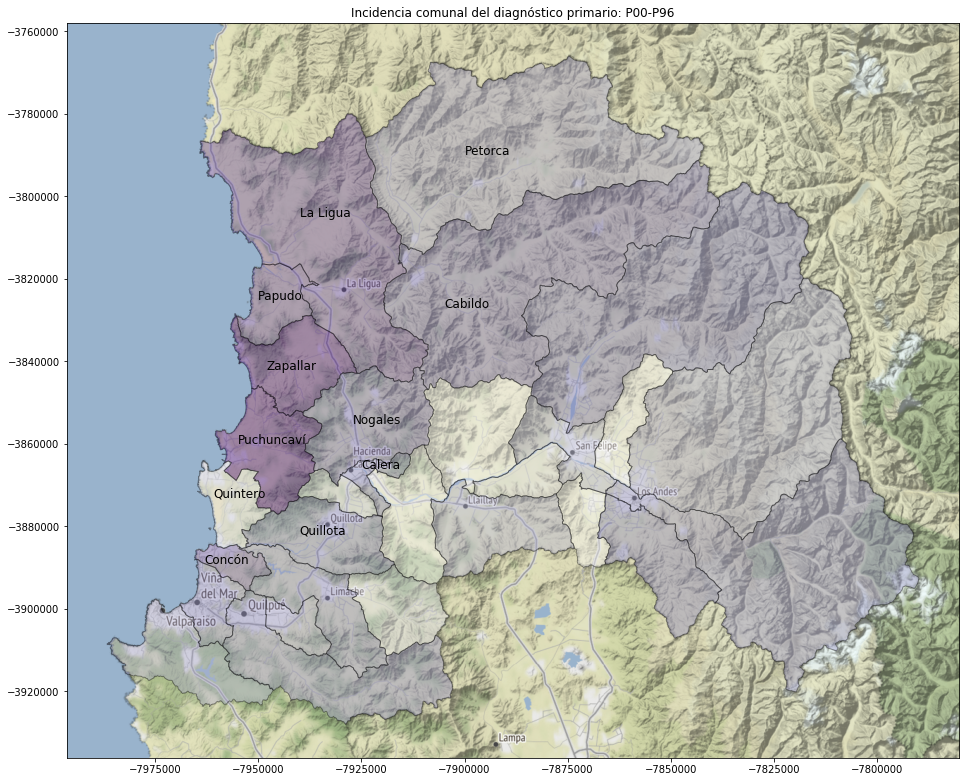
\includegraphics{assets/mapa.png}
\caption{Figura 2: Mapa de incidencias comunales}
\end{figure}

\hypertarget{se-observa-una-distribuciuxf3n-no-radial-cuxf3mo-se-explica}{%
\subsubsection{Se observa una distribución no-radial: ¿Cómo se
explica?}\label{se-observa-una-distribuciuxf3n-no-radial-cuxf3mo-se-explica}}

En la figura 2 se puede apreciar que las comunas más afectadas parecen
ser las directamente al norte (Puchuncaví, Zapallar, Papudo y La Ligua),
al este (Nogales, La Calera y Quillota) e incluso directamente al sur
(Concón) del complejo industrial.

Al observar esta distribución no radial, la investigación parecía no
tener sentido y se estancó durante un tiempo. Se sospechaba de un patrón
de vientos. Para seguir avanzando, fue necesario que se nos refiriera a
la investigación de Patricio Cornejo, Juan López y Sergio Romano
1983\textsuperscript{{6}}, donde se creó un mapa que indica la
dispersión de contaminación desde el complejo industrial
Quintero-Ventanas.

Al sobreponer ese mapa sobre nuestras incidencias (Figura 3), observamos
una coincidencia interesante, que nos llevó a continuar.

\begin{figure}
\centering
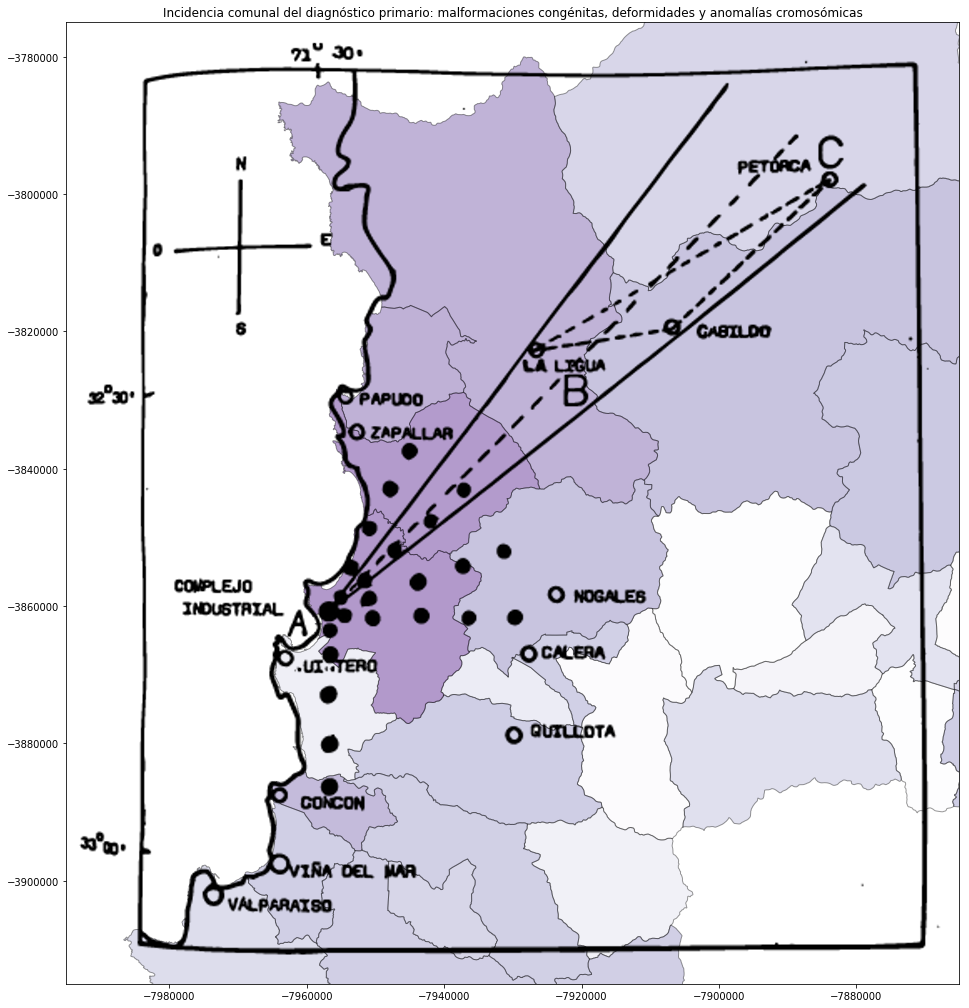
\includegraphics{assets/mapa-pluma.png}
\caption{Figura 3: Mapa de incidencias comunales con modelo pluma (Cornejo, López y Romano 1983)
sobrepuesto}
\end{figure}

\hypertarget{diferentes-zonas-de-interuxe9s}{%
\subsubsection{Diferentes zonas de
interés}\label{diferentes-zonas-de-interuxe9s}}

Debido a que el mapa y la incidencia de Q00-Q99 parecieran indicar en la
dirección opuesta de la ciudad de Quintero, y la sospecha de que Concón
tenga su propia fuente de contaminación (Refinería de petróleo ENAP),
analizamos tres grupos en paralelo: El primero excluyendo Concón y
Quintero, el segundo incluyendo ambas comunas, y el tercero incluyendo
Concón y excluyendo Quintero.

A continuación, graficamos la incidencia del diagnóstico primario en estos grupos e imprimimos
algunos indicadores de representatividad como tamaño del grupo, y
cuántos de sus diagnósticos primarios están entre los 10 principales que
graficamos.

\begin{verbatim}
Grupo 1
Zona de interés: Puchuncaví, Zapallar, Papudo, La Ligua, Petorca, Cabildo, Nogales
Total defunciones en el grupo de interés: 313
Total defunciones en los 10 principales diagnósticos primarios del grupo de interés: 308
Fracción del total: 0.984
\end{verbatim}

\begin{figure}
\centering
\textbf{Grupo 1}\par\medskip
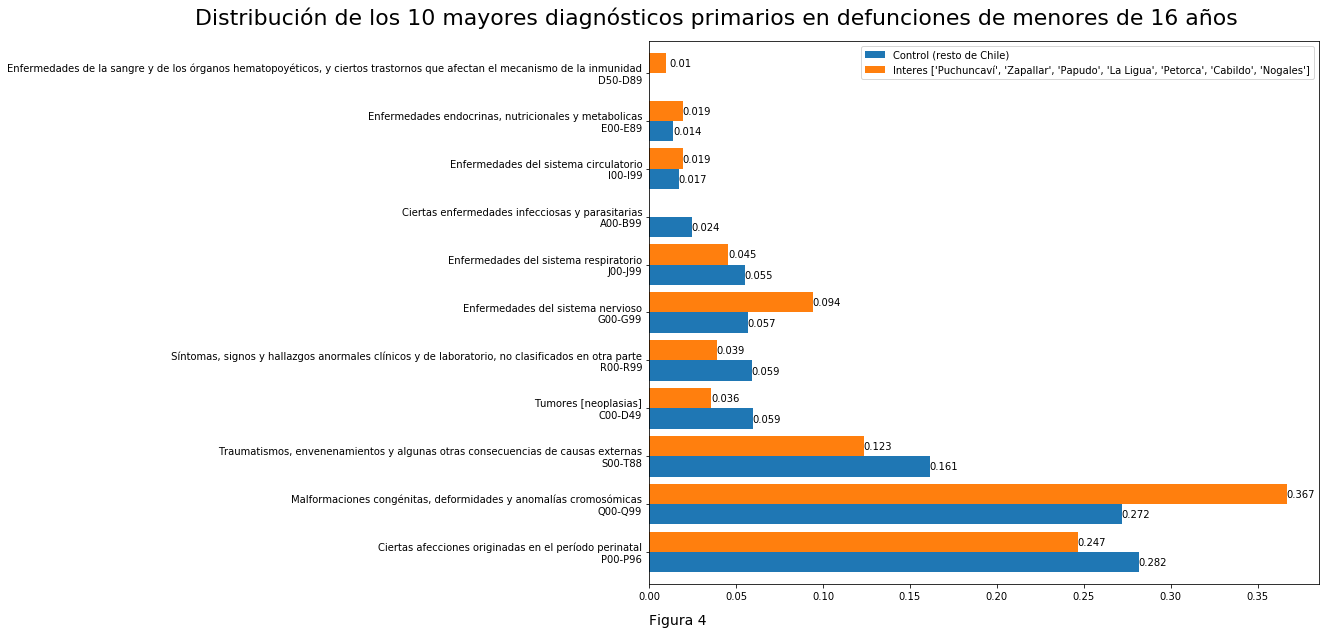
\includegraphics{assets/10-diagnosticos-(Puchuncavi-Zapallar-Papudo-LaLigua-Petorca-Cabildo-Nogales).png}
\caption{Figura 4: Distribución de los 10 mayores diagnósticos primarios en defunciones de menores hasta 16 años (Puchuncaví-Zapallar-Papudo-La Ligua-Petorca-Cabildo-Nogales)}
\end{figure}

\begin{verbatim}
Grupo 2
Zona de interés: Puchuncaví, Zapallar, Papudo, La Ligua, Petorca, Cabildo, Nogales, Concón, Quintero
Total defunciones en el grupo de interés: 471
Total defunciones en los 10 principales diagnósticos primarios del grupo de interés: 462
Fracción del total: 0.981
\end{verbatim}

\begin{figure}
\centering
\textbf{Grupo 2}\par\medskip
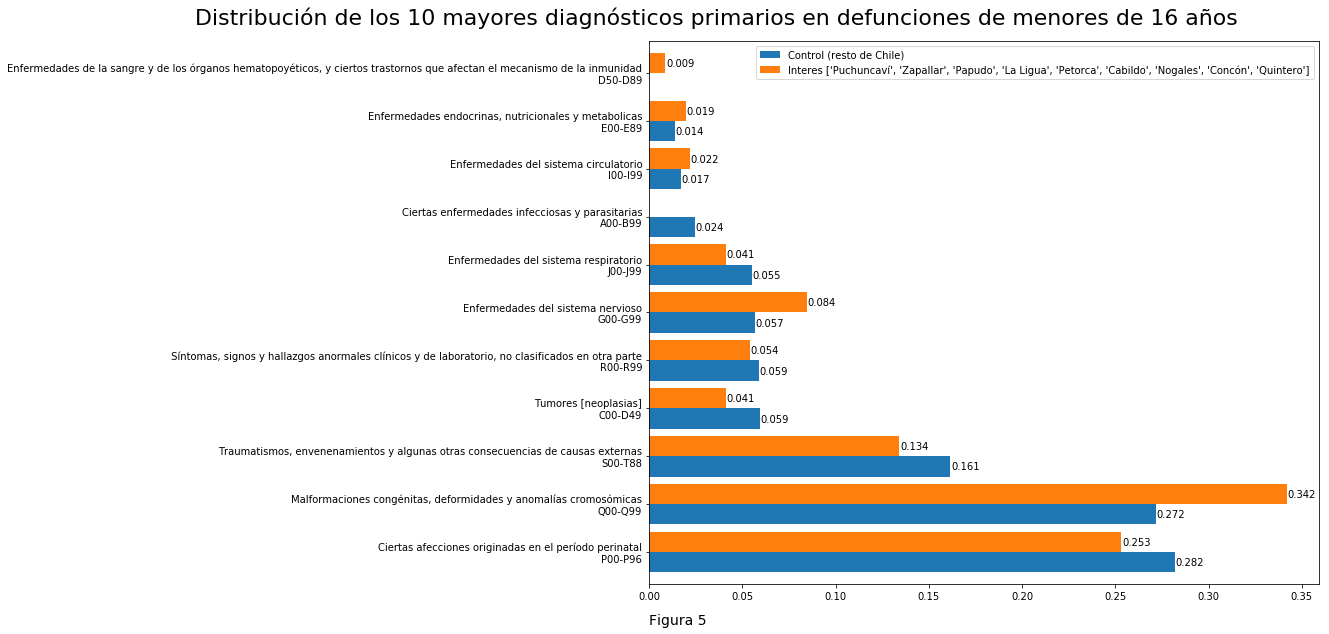
\includegraphics{assets/10-diagnosticos-(Puchuncavi-Zapallar-Papudo-LaLigua-Petorca-Cabildo-Nogales-Concon-Quintero).png}
\caption{Figura 5: Distribución de los 10 mayores diagnósticos primarios en defunciones de menores hasta 16 años Puchuncaví-Zapallar-Papudo-La Ligua-Petorca-Cabildo-Nogales-Concón-Quintero)}
\end{figure}

\begin{verbatim}
Grupo 3
Zona de interés: Puchuncaví, Zapallar, Papudo, La Ligua, Petorca, Cabildo, Nogales, Concón
Total defunciones en el grupo de interés: 398
Total defunciones en los 10 principales diagnósticos primarios del grupo de interés: 390
Fracción del total: 0.980
\end{verbatim}

\begin{figure}
\centering
\textbf{Grupo 3}\par\medskip
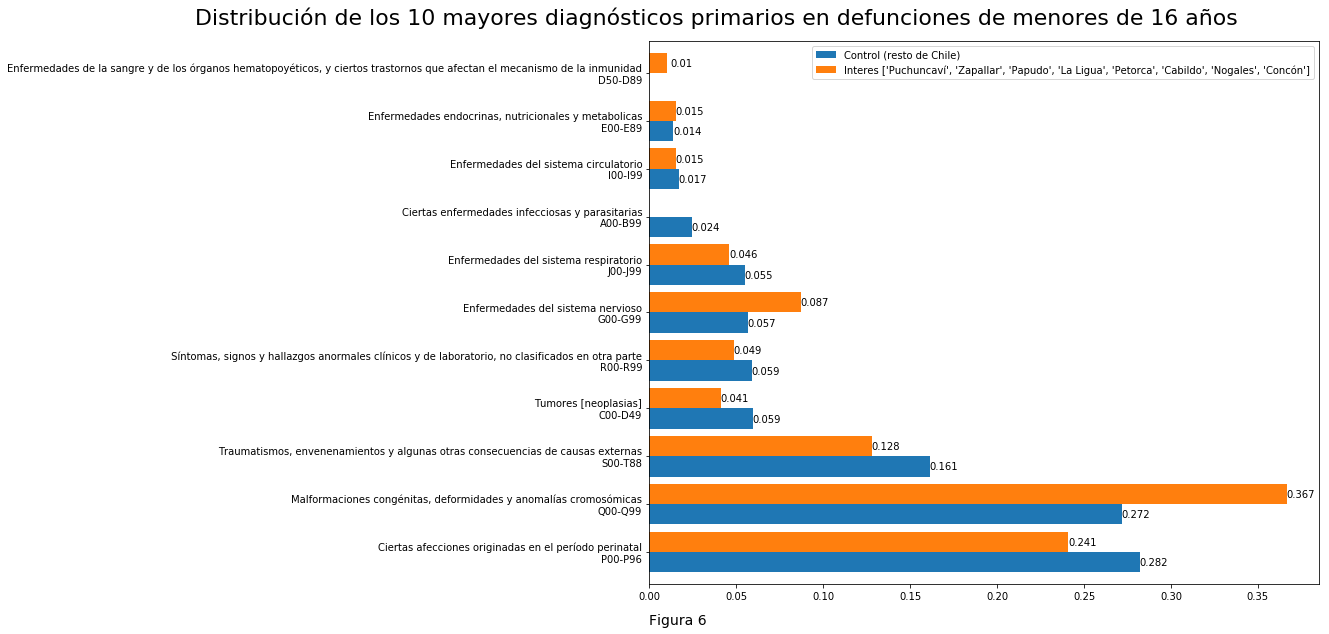
\includegraphics{assets/10-diagnosticos-(Puchuncavi-Zapallar-Papudo-LaLigua-Petorca-Cabildo-Nogales-Concon).png}
\caption{Figura 6: Distribución de los 10 mayores diagnósticos primarios en defunciones de menores hasta 16 años (Puchuncaví-Zapallar-Papudo-La Ligua-Petorca-Cabildo-Nogales-Concón)}
\end{figure}

\hypertarget{observaciones}{%
\subsection{Observaciones}\label{observaciones}}

Al comparar estos gráficos, inmediatamente notamos que el diagnóstico
primario \emph{Malformaciones congénitas, deformidades y anomalías
cromosómicas} (CIE-10: Q00-Q99), es considerablemente más alto en los
grupos de interés que en el resto del país como grupo de control
(36.7\%, 34.2\% y 36.7\% por sobre 27.2\%).

\hypertarget{validaciuxf3n}{%
\subsection{Validación}\label{validaciuxf3n}}

Para validar estas observaciones realizamos una prueba de permutación:

Por cada grupo, tomamos un millón de muestras al azar del mismo tamaño que el
grupo de interés (308, 471 y 398) desde el grupo de control, y
observaremos la distribución del diagnóstico primario de interés en
estas muestras, en contraste con casos seleccionados por zona geografía de interés, a fin de responder:

\textbf{¿Qué tan probable es observar las incidencias (36.7\%, 34.2\% y
36.7\%) que se dan en nuestros grupos de interés en cualquier otro grupo
del mismo tamaño muestreado al azar desde el grupo de control?}

\begin{figure}
\centering
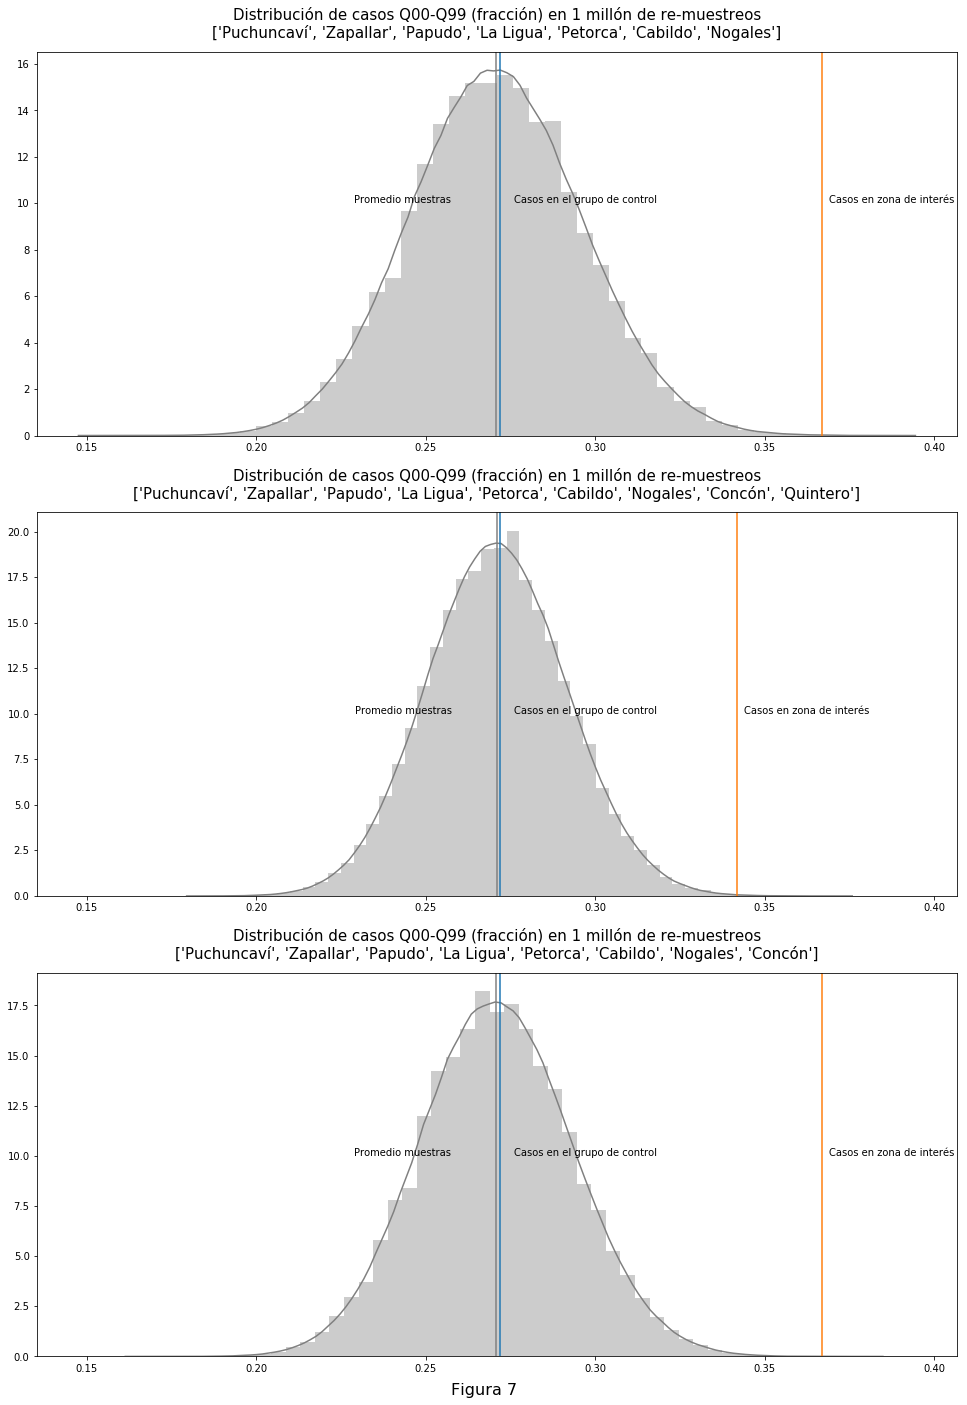
\includegraphics{assets/distribucion.png}
\caption{Figura 7: Distribución fracción de casos Q00-Q99 en 1 millón de re-muestreos}
\end{figure}

\hypertarget{otros-valores-de-interuxe9s}{%
\subsection{Otros valores de
interés}\label{otros-valores-de-interuxe9s}}

En la figura 7 podemos ver la ubicación de las incidencias observadas
(línea naranja) con la distribución en el grupo de control del
diagnóstico primario \emph{malformaciones congénitas, deformidades y
anomalías cromosómicas}.

A continuación cuantificamos la observación anterior con los siguientes
números:

\begin{itemize}
\tightlist
\item
  Probabilidad de obtener este resultado, o más, al azar (p-value)
\item
  Incidencia promedio en muestras al azar desde el grupo de control
\item
  Desviación estándar de muestras al azar desde el grupo de control
\item
  Cuantificación en desviaciones estándar respecto del grupo de control, desde los grupos en el promedio de un millón de re-muestreos
\end{itemize}

\begin{verbatim}
Grupo 1
['Puchuncaví', 'Zapallar', 'Papudo', 'La Ligua', 'Petorca', 'Cabildo', 'Nogales']
P-value: 0.00010
Promedio de las muestras: 0.27083
Desviación standard de las muestras: 0.02528
Distancia entre el promedio de las muestras y el grupo de interés en desviaciones standard: 3.05

Grupo 2
['Puchuncaví', 'Zapallar', 'Papudo', 'La Ligua', 'Petorca', 'Cabildo', 'Nogales', 'Concón', 'Quintero']
P-value: 0.00039
Promedio de las muestras: 0.27103
Desviación standard de las muestras: 0.02059
Distancia entre el promedio de las muestras y el grupo de interés en desviaciones standard: 3.74

Grupo 3
['Puchuncaví', 'Zapallar', 'Papudo', 'La Ligua', 'Petorca', 'Cabildo', 'Nogales', 'Concón']
P-value: 0.00002
Promedio de las muestras: 0.27085
Desviación standard de las muestras: 0.02239
Distancia entre el promedio de las muestras y el grupo de interés en desviaciones standard: 3.45
\end{verbatim}

\hypertarget{variaciones-en-el-p-value}{%
\subsection{Variaciones en el P-value}\label{variaciones-en-el-p-value}}

A razón de haber observado variaciones en el primer dígito no-cero del
p-value durante las primeras ejecuciones de 10.000 re-muestreos, se aumento
la cantidad de re-muestreos en dos órdenes de magnitud (a un millón). Y para entender
como se comporta este p-value respecto a la cantidad de re-muestreos,
tomamos sub-muestras del millón de muestras, incrementando su tamaño iterativamente en 500 re-muestreos. Al
graficar el p-value en estos distintos tamaños de re-muestreos, se
observa que en el n inicial de 10.000 el p-value se lograba estabilizar en su orden
de magnitud, pero con un millón se estabilizaba considerablemente más.

\begin{figure}
\centering
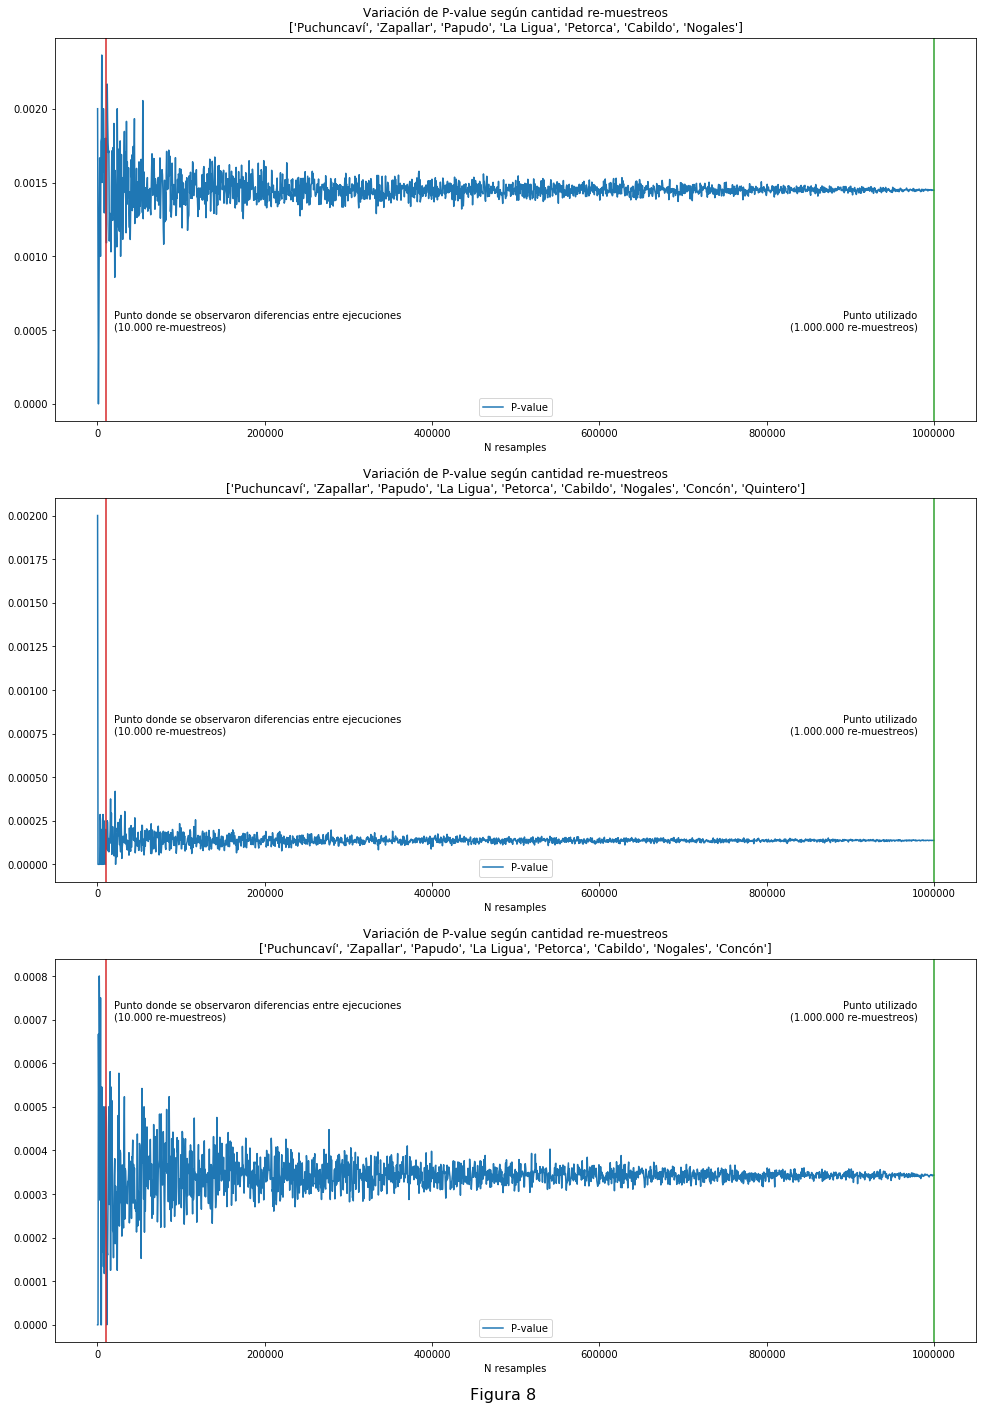
\includegraphics{assets/variacion-p-values.png}
\caption{Figura 8: Variaciones en P-values sobre cantidad de simulaciones}
\end{figure}

\hypertarget{conclusiones}{%
\subsection{Conclusiones}\label{conclusiones}}

\begin{longtable}[]{@{}llll@{}}
\toprule
\begin{minipage}[b]{0.22\columnwidth}\raggedright
Grupo\strut
\end{minipage} & \begin{minipage}[b]{0.22\columnwidth}\raggedright
Distancia DS\strut
\end{minipage} & \begin{minipage}[b]{0.22\columnwidth}\raggedright
P-Value\strut
\end{minipage} & \begin{minipage}[b]{0.22\columnwidth}\raggedright
Comunas\strut
\end{minipage}\tabularnewline
\midrule
\endhead
\begin{minipage}[t]{0.22\columnwidth}\raggedright
1\strut
\end{minipage} & \begin{minipage}[t]{0.22\columnwidth}\raggedright
3.05\strut
\end{minipage} & \begin{minipage}[t]{0.22\columnwidth}\raggedright
0.00010\strut
\end{minipage} & \begin{minipage}[t]{0.22\columnwidth}\raggedright
{[}`Puchuncaví', `Zapallar', `Papudo', `La Ligua', `Petorca', `Cabildo',
`Nogales'{]}\strut
\end{minipage}\tabularnewline
\begin{minipage}[t]{0.22\columnwidth}\raggedright
2\strut
\end{minipage} & \begin{minipage}[t]{0.22\columnwidth}\raggedright
3.74\strut
\end{minipage} & \begin{minipage}[t]{0.22\columnwidth}\raggedright
0.00039\strut
\end{minipage} & \begin{minipage}[t]{0.22\columnwidth}\raggedright
{[}`Puchuncaví', `Zapallar', `Papudo', `La Ligua', `Petorca', `Cabildo',
`Nogales', `Concón', `Quintero'{]}\strut
\end{minipage}\tabularnewline
\begin{minipage}[t]{0.22\columnwidth}\raggedright
3\strut
\end{minipage} & \begin{minipage}[t]{0.22\columnwidth}\raggedright
3.45\strut
\end{minipage} & \begin{minipage}[t]{0.22\columnwidth}\raggedright
0.00002\strut
\end{minipage} & \begin{minipage}[t]{0.22\columnwidth}\raggedright
{[}`Puchuncaví', `Zapallar', `Papudo', `La Ligua', `Petorca', `Cabildo',
`Nogales', `Concón'{]}\strut
\end{minipage}\tabularnewline
\bottomrule
\caption{Tabla 3: desviaciones estándar por sobre el resto del país de los grupos y su p-value}
\end{longtable}

Tales distancias (3.05, 3.74 y 3.45 desviaciones estándar) entre los
valores observados y los promedios del grupo de control (figura 7), así
como los p-values observados en el millón de re-muestreos por grupo y su
estabilidad observada (figura 8), muestran \textbf{una cifra de mortalidad anómala en la zona en estudio}.

Si le restamos la incidencia nacional esperada \emph{(0.272 * 313, 0.272
* 471, 0.272 * 398)} a los grupos de análisis \emph{(0.367 * 313, 0.342
* 471, 0.367 * 398)} podremos estimar que \textbf{estamos observando 29.73,
32.97 o 37.8 muertes de menores hasta 16 años en las zonas analizadas, que
no observaríamos en el resto de Chile a igual tamaño de muestra}, en el
periodo 1998-2016.

Se recomienda enfáticamente seguir observando estos números mientras la
fuente de contaminación siga ahí, y durante dos a tres décadas después
de que el complejo industrial sea clausurado y la zona, descontaminada.

Se invita a los expertos de las áreas relevantes (salud, bioquímica,
ecología, etc.) a investigar la rutas específicas que llevarían al
incremento de las defunciones bajo este diagnóstico primario. Se invita,
además, a los gobernantes a hacer la prueba de campo, clausurando las
fuentes y descontaminando el área, para observar, en algunas décadas, la
evolución de la incidencia de este diagnóstico primario en las
defunciones de la zona.

\hypertarget{potencial-futuro-de-la-metodologuxeda}{%
\subsubsection{Potencial futuro de la
metodología}\label{potencial-futuro-de-la-metodologuxeda}}

Esta técnica puede ser escalada a nivel nacional para buscar otros
fenómenos del mismo tipo, sin especificar una zona en particular, lo que
podría revelar problemas de salud pública fuera del ``radar'' de los
investigadores. Para esto se requeriría construir un graph con comunas
como nodos, y sus colindacias geográficas como vértices (tal vez con
\href{https://www.bcn.cl/siit/mapas_vectoriales/index_html}{los vectores
de comunas de la biblioteca del congreso}), e iterar sobre grupos de
comunas colindantes con un mínimo de registros totales. De realizarse,
se sugiere nombrar \emph{Perico} a tal algoritmo que \emph{treparía por
Chile}.

\hypertarget{agradecimientos}{%
\subsubsection{Agradecimientos}\label{agradecimientos}}

Al Dr. Yuri Carvajal por la orientación bibliográfica, corrección e implementación de LaTeX. Y a la biblioteca Gabriela Mistral de Ñuñoa por haber sido mi "universidad anfitriona" durante los meses de esta investigación.


\hypertarget{refs}{%
\subsubsection{Referencias}\label{referencias}}

\leavevmode\hypertarget{defunciones-decoder}{}%
1. https://github.com/verasativa/defunciones-decoder

\leavevmode\hypertarget{codigo-fuente}{}%
2. https://github.com/verasativa/zonacritica/

\leavevmode\hypertarget{ref-cms59}{}%
3. Salud \& ambiente: Geografías en sacrificio. Vol. 59, Cuadernos
Médico Sociales (Chile). 2019.

\leavevmode\hypertarget{ref-landrigan2017}{}%
4. Philip J Landrigan NJRA Richard Fuller. The lancet commission on
pollution and health. \emph{The Lancet}. 2018;391(10119):475.

\leavevmode\hypertarget{CIE-10}{}%
5. https://github.com/verasativa/CIE-10/

\leavevmode\hypertarget{ref-cms80s}{}%
6. Cavieres MF. Estudios sobre la contaminación de puchuncaví en la
decada de los 80. Un aporte científico que no fue. \emph{Cuadernos
Médico Sociales (Chile)}. 2019;59(1):35.

\end{document}
